\chapter{Design} \label{chapter:design}

In this chapter, we describe the design and algorithms that discipline the
operation of the Cluster Autoscaler and the Scheduler; we point out their
shortcomings concerning local data storage and propose design enhancements to
enable seamless scheduling and autoscaling with local persistent volumes.

\section{Design Rationale \& Goals}

As explained in section \ref{section:intro_problem_statement}, our goal is to
extend the Scheduler and the Cluster Autoscaler so that they operate seamlessly
with workloads that use volumes backed by local storage. More specifically, we
aim to:

\begin{itemize}
      \tightlist
      \item Extend the Scheduler to consider the storage capacity of the nodes
            when scheduling Pods.
      \item Extend the Autoscaler to scale-down nodes where local volumes live,
            ensuring that Rok's mechanism snapshots the data before removing the
            node from the cluster.
      \item Extend the Autoscaler to check if the Pod's volumes can be placed on
            any other node (with regards to storage capacity) when evaluating (for
            a possible scale-down) if a Pod can be moved elsewhere.
      \item Extend the Autoscaler to consider the storage capacity of nodes, and,
            when scaling up, add a node with enough storage capacity.
      \item Extend the Autoscaler to not remove unready nodes in case local
            volumes live on these nodes.
\end{itemize}

\section{Rok's Local Volume Mechanism}

Local data on a node need a mechanism to be backed up if the node gets removed
from the cluster; otherwise, the data will be permanently lost, and the user
will not be able to recover them.

Rok provides a mechanism that enables the functionality of moving volumes around
the nodes of a cluster. It leverages an external storage system, such as
Amazon's S3, where it snapshots the local volumes and can restore them on a
different node. Rok refers to moving a local volume to Amazon S3 as
\textit{``Unpinning''} and restoring the volume to a different node as
\textit{``Pinning''}. We describe this mechanism in greater depth in the
following section.

\subsection{Rok Volume Pinning and Unpinning}

\label{section:rok-volume-pinning}

When a local volume is provisioned on a node, the corresponding
\co{PersistentVolume} object on the API Server that represents the volume has
node affinity on it (see section \ref{section:background-pv-node-affinity}). In
the case of local storage, the Rok CSI driver sets the node affinity of the PV
to match only with the node where the local volume is provisioned.


Rok introduces the following terms:
\begin{itemize}
	\tightlist

	\item \textit{Pinned PV}: A PV representing a node's local volume. This PV
	      has node affinity to indicate that it is accessible only from that
	      particular node.
	\item \textit{Unpinned PV}: A PV representing a local volume migrated to S3.
	      The PV has an empty node affinity to indicate that it is accessible
	      from every cluster node.
\end{itemize}

A pinned PV can become unpinned with the process of ``\textit{unpinning}''. An
unpinned PV can become pinned with the process of ``\textit{pinning}''. The
process can be repeated multiple times, essentially allowing the volume to move
around the cluster nodes as many times as needed.

\label{section:design-unpin}
The Rok CSI Controller implements the following mechanism for the unpinning of a
PV:
\begin{enumerate}
	\tightlist
	\item Watches for nodes that are marked unschedulable.
	\item Finds volumes on the unschedulable node that are not currently used by
	      any Pods.
	\item Starts the unpinning process of the unused PV: it takes snapshots of
	      the volume on Amazon S3.
	\item Removes the node affinity from the PV. Note that the \co{nodeAffinity}
	      field of a PV is immutable, i.e., it is not allowed to change. To
	      overcome this restriction, Rok deletes the PV and instantaneously
	      recreates it.
\end{enumerate}

Rok implements the following mechanism for the pinning of a PV:
\begin{enumerate}
	\tightlist
	\item The Scheduler schedules the Pod that references the unpinned PV
	      (through a PVC).
	\item The Kubernetes \co{attachDetach} controller creates a
	      \co{VolumeAttachment} object to signal the external attacher to attach
	      the volume on the node.
	\item The external attacher sees the VolumeAttachment and issues a
	      \co{ControllerPublishVolume} call to the Rok CSI controller.
	\item The Rok CSI controller creates a logical volume on the Rok VG and
	      restores the data of the PV from the Amazon S3 to the logical volume.
	\item The Rok CSI controller sets the appropriate node affinity on the PV to
	      indicate its only accessible from the node the volume was restored to.
\end{enumerate}


\subsection{Rok's Local Volume Protection Mechanism}
\label{section:background-rok-csi-guard}

The Kubernetes maintenance and upgrade tools rely on the \co{drain} operation
(see \ref{section:cordon-drain}). Essentially, before taking any actions to
remove or upgrade a node in the cluster, the tools drain the node (\co{kubectl
	drain}) in order to mark the node unschedulable and safely evict all the Pods.
The Cluster Autoscaler also uses the drain operation before removing a node.

Rok deploys a mechanism to facilitate the upgrades of a cluster and ensure that
the nodes are not removed before Rok snapshots all their local volumes.

The mechanism leverages Pods with properly configured PodDisruptionBudgets to
block their eviction. It relies on the fact that the drain operation fails as
long as the eviction of a Pod fails. The mechanism works as follows:

\begin{enumerate}
	\tightlist
	\item The Rok Operator creates a \co{Deployment} resource \textit{for each
		      node} in the cluster. The Deployment of each node creates
	      \textit{exactly} one replica Pod with node affinity that matches
	      only the specific node. Rok names these Pods  ``\textit{CSI Guard
		      Pod}'', since they protect the node's local volumes.
	\item The Rok Operator creates a \co{PodDisruptionBudget} object for each
	      Rok CSI Guard Deployment. The PodDisruptionBudget demands at any time
	      to exist at least one Rok CSI Guard Pod of the Deployment. This
	      configuration causes any evictions of the Rok CSI Guard Pod to fail.
	\item The drain operation marks the node unschedulable and starts evicting
	      the Pods on the node. The eviction of the CSI Guard fails because of
	      the configured PodDisruptionBudget.
	\item The Rok Operator checks if the Rok CSI has unpinned all the volumes of
	      the unschedulable node; if this condition holds, it removes the
	      PodDisruptionBudget that corresponds to the CSI Guard of the node.
	\item Since the PodDisruptionBudget does not exist anymore, the eviction of
	      the  Rok CSI Guard Pod finally succeeds, and the drain operation
	      completes.
\end{enumerate}

The mechanism is illustrated in Figure ~\ref{figure:rok-csi-guards}.

\clearpage
\vspace*{2cm}
\begin{figure}[H]
	\centering
	\makebox[\textwidth][c]{
		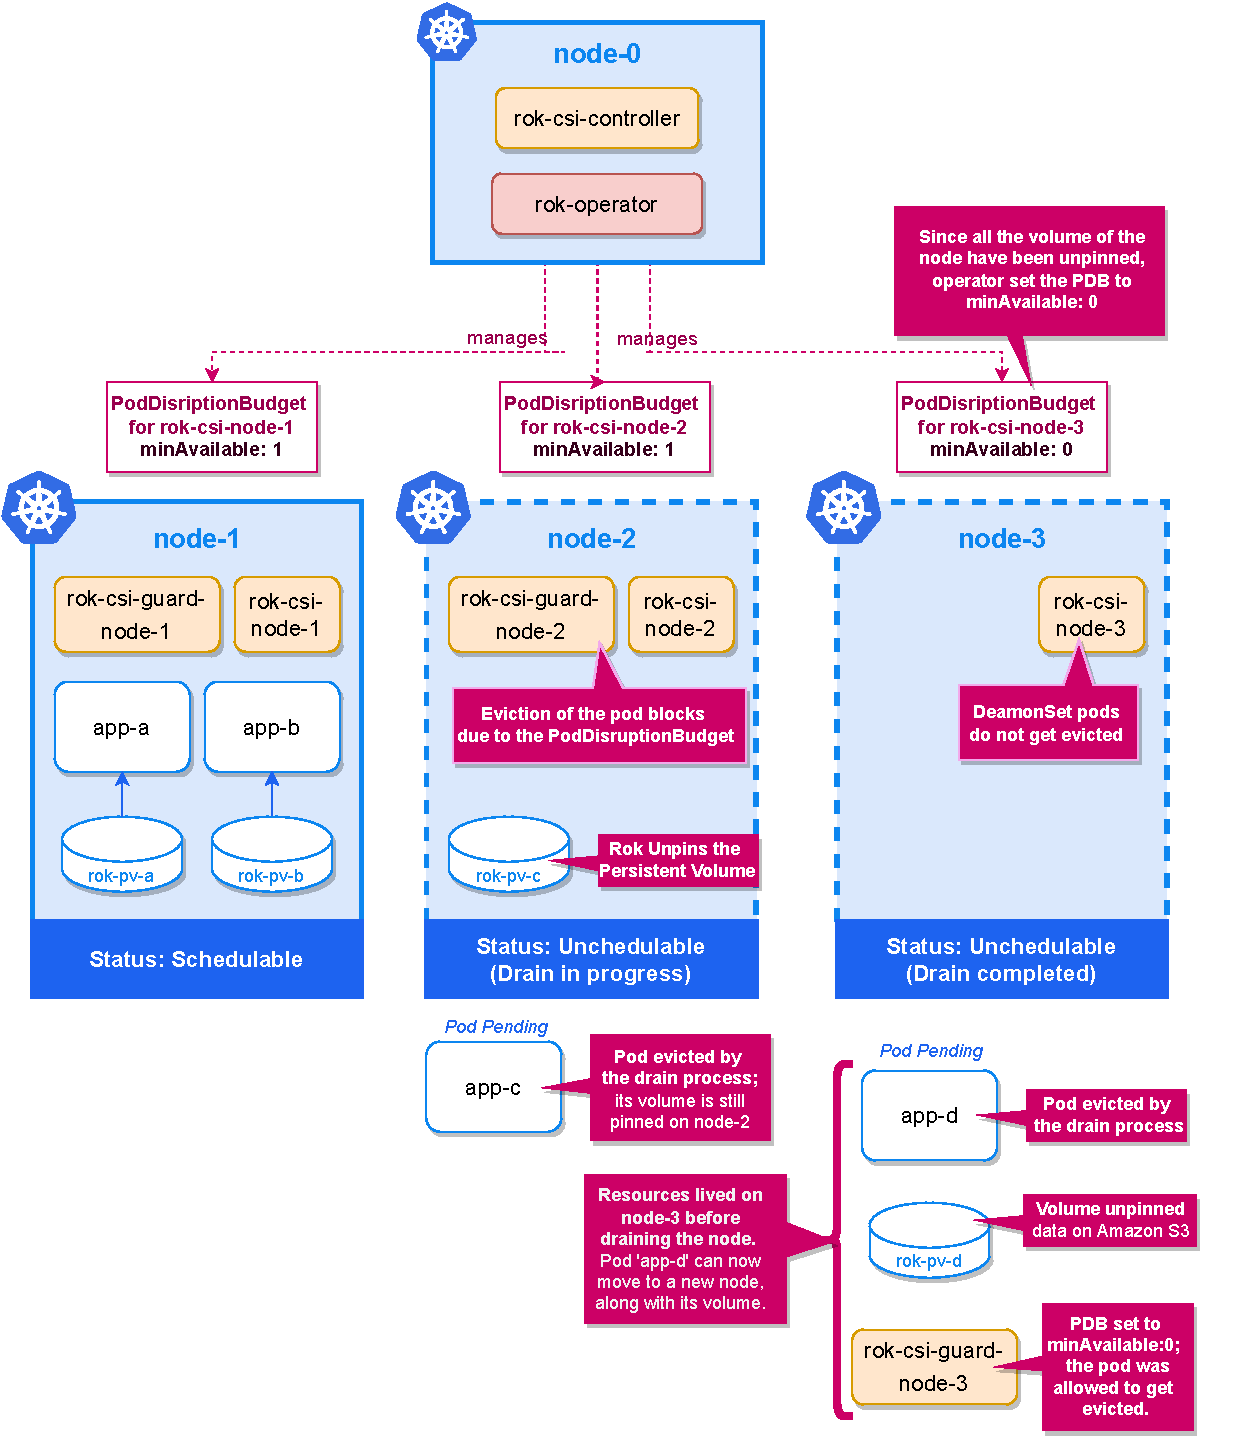
\includegraphics[width=1.2\textwidth]{resources/drain-cluster.pdf}
	}
	\caption{Protecting Local Data with Rok CSI Guard Pods}
	\label{figure:rok-csi-guards}
\end{figure}
\clearpage
\section{Kubernetes Scheduler}
\RestyleAlgo{ruled}

Σε αυτήν την ενότητα, θα παρουσιάσουμε συνοπτικά τη τρέχουσα σχεδίαση του
Kubernetes Scheduler, θα επισημάνουμε τις ελλείψεις που υπάρχουν και θα
προτείνουμε βελτιώσεις που επιλύουν τους τρέχοντες περιορισμούς.

\subsection{To Πρόσθετο VolumeBinding}

Για λόγους συντομίας, στο ελληνικό τμήμα της διπλωματικής παρουσιάζουμε μόνο τη
σχεδίαση της \co{Filter} και της \co{PreBind}  φάσης του προσθέτου, καθώς
σχετίζεται άμεσα με τις προτεινόμενες επεκτάσεις. Για την αναλυτική παρουσίαση
των υπολοίπων φάσεων του προσθέτου, μπορείτε να ανατρέξετε στο αντίστοιχο
αγγλικό κεφάλαιο, στην ενότητα \ref{section:design-volume-binding}.

\subsection*{PreFilter Φάση}

\co{Filter}: αξιολογεί αν ένα Pod μπορεί να τοποθετηθεί σε έναν κόμβο, βάσει των
τόμων που ζητά, τόσο για τα δεσμευμένα όσο και για τα μη δεσμευμένα PVC:
\begin{itemize}
      \tightlist
      \item Για τα \textit{δεσμευμένα PVC}, ελέγχει ότι το PV του κάθε PVC είναι
            προσβάσιμο (βάσει τoy node affinity που φέρει) από τον εξεταζόμενο
            κόμβο.
      \item Για τα \textit{μη δεσμευμένα PVC}, προσπαθεί να βρει διαθέσιμα PVs
            που μπορούν να ικανοποιήσουν τις απαιτήσεις του PVC και που είναι
            προσβάσιμα (βάσει του node affinity τους) από τον εξεταζόμενο κόμβο.
            Τα PVCs για τα οποία δεν κατάφερε να βρει κατάλληλα PVs, θα τα
            αποκαλούμε εφεξής ``\textit{PVCs to provision}''.
      \item Για κάθε \textit{PVC to provision}, ελέγχει αν η \co{StorageClass}
            του PVC υποστηρίζει τη δυναμική παροχή και αν υπάρχει αρκετή
            χωρητικότητα αποθήκευσης προσβάσιμη από τον κόμβο. Εάν όχι, το Pod
            δεν μπορεί να ανατεθεί στον κόμβο. Αυτό είναι το βήμα όπου
            η χωρητικότητα αποθήκευσης λαμβάνεται υπόψη.

\end{itemize}

Η τρέχουσα υλοποίηση του χρονοδρομολογητή, ελέγχει αν υπάρχει αρκετή
χωρητικότητα για κάθε PVC to provision, καλώντας τη μέθοδο \co{hasEnough()} με
ένα μόνο PVC ως είσοδο. Ζητά από τον  API Server όλα τα αντικείμενα
\co{CSIStorageCapacity}. και ελέγχει αν κάποιο από αυτά ταιριάζει με το
\co{StorageClass} του PVC, είναι προσβάσιμο από τον εξεταζόμενο κόμβο και η
αναφερόμενη χωρητικότητα του αντικειμένου είναι μεγαλύτερη από τη ζητούμενη
χωρητικότητα του PVC. Εάν ένα τέτοιο CSIStorageCapacity υπάρχει, υπάρχει αρκετός
χώρος στον κόμβο για τη δυναμική παροχή τόμου για το εξεταζόμενο PVC.

Είναι σημαντικό να επισημάνουμε ότι δεν ελεγχει αν υπάρχει αποθηκευτικός χώρος
συνολικά για όλα τα PVCs, αλλά μόνο αν το κάθε PVC χωριστά χωράει σε έναν κόμβο.

\subsection*{PreBind Φάση}

Η φάση \co{PreBind} εκτελείται αφού ο χρονοδρομολογητής έχει επιλέξει έναν κόμβο
για  το Pod.

Για κάθε ένα από τα \textit{μη δεσμευμένα PVC} που το πρόσθετο βρήκε ένα
κατάλληλο PV κατά τη διάρκεια της φάσης \co{Filter}, θα ενημερώσει τον API
Server με τη δέσμευση, δηλαδή, θα ενημερώσει το αντίστοιχο PV ώστε να δείχνει
στο PVC, και στη συνέχεια, ο ελεγκτής Kubernetes PersistentVolume θα ολοκληρώσει
την αμφίδρομη δέσμευση.

Για κάθε ένα από τα \textit{PVCs to provision}, θα ενημερώσει τα αντίστοιχα PVCs
στον API Server με το  ``selected node annotation'' \footnote{Το selected node
annotation: \co{volume.kubernetes.io/selected-node}} για να σηματοδοτήσει στον
\en{external provisioner} ότι ένας τόμος για το PVC πρέπει να δημιουργηθεί δυναμικά
σε ένα τμήμα τοπολογίας που είναι προσβάσιμο από τον κόμβο που υποδεικνύει η
σημείωση. 

Στη συνέχεια, το πρόσθετο θα κάνει poll τον API Server έως ότου όλα τα PVCs
δεσμευτούν  PVs. Εάν το selected node annotation κάποιου PVC to provision
αφαιρεθεί, θα ακυρώσει την τρέχουσα προσπάθεια χρονοδρομολόγησης και θα
καλέσει τα πρόσθετα \co{Unreserve}.Η αφαίρεση του annotation είναι ένας
μηχανισμός με τον οποίο ο external provisioner ουσιαστικά ειδοποιεί τον
χρονοδρομολογητή ότι απέτυχε η παροχή του τόμου και θα πρέπει να δοκιμάσει ξανά,
ενδεχομένως σε άλλον κόμβο.


\subsection{Ελλείψεις \& Προτεινόμενες Επεκτάσεις}

Σύμφωνα με την προηγούμενη ανάλυση των αλγορίθμων, ο τρέχων σχεδιασμός του
Kubernetes Scheduler έχει τους ακόλουθους περιορισμούς:

\begin{enumerate}
      \item Η μέθοδος \texttt{Filter} του πρόσθετου VolumeBinding χρησιμοποιεί
            τα αντικείμενα \en{CSIStorageCapacity} του Kubernetes API για να
            αντλήσει πληροφορίες για τον διαθέσιμο αποθηκευτικό χώρο. Αυτό το
            αντικείμενο API έγινε beta στην έκδοση Kubernetes 1.21 και ήταν σε
            κατάσταση alpha σε προηγούμενες εκδόσεις. Οι κύριοι πάροχοι
            υπηρεσιών νέφους δεν ενεργοποιούν τα χαρακτηριστικά σε κατάσταση
            alpha στις υπηρεσίες τους. Ως αποτέλεσμα, τα CSIStorageCapacity
            αντικείμενα δεν είναι ενεργοποιημένα σε συστοιχίες που εκτελούν
            εκδόσεις προγενέστερες της 1.21 στους περισσότερους παρόχους cloud.
            Αυτό είναι ένα σημαντικό πρόβλημα, δεδομένου ότι πολλές επιχειρήσεις
            (συμπεριλαμβανομένων των πελατών μας) δεν τρέχουν τις τελευταίες
            εκδόσεις του Kubernetes για λόγους σταθερότητας. Στη δική μας
            περίπτωση, οι πελάτες μας εκτελούν συστοιχίες Kubernetes 1.19 και
            1.20 και χρειάζονταν τη δυνατότητα χρονοδρομολόγησης Pods με εξέταση
            της τοπικής αποθήκευσης.
      \item Η τρέχουσα σχεδιαστική λογική της φάσης \co{Filter} του πρόσθετου
            \co{VolumeBinding} δεν λαμβάνει υπόψη της τον αποθηκευτικό χώρο που
            απαιτείται για την παροχή πολλαπλών PVC ενός Pod. Αντ' αυτού,
            ελέγχει αν κάθε μεμονωμένο PVC μπορεί να δημιουργηθεί στον
            αποθηκευτικό χώρο που είναι προσβάσιμος από τον κόμβο, χωρίς να
            διασφαλίζει ότι υπάρχει αρκετός χώρος για όλα αυτά ταυτόχρονα. Αυτό
            είναι ένα κρίσιμο πρόβλημα: σε περίπτωση που ένα Pod αναφέρεται σε
            πολλαπλά μη δεσμευμένα PVC και δεν υπάρχει αρκετός χώρος για όλα
            αυτά, ένα από αυτά γίνει provision και η παροχή των υπολοίπων θα
            αποτύχει, τότε όλες οι μελλοντικές αποφάσεις χρονοδρομολόγησης θα
            περιορίζονται από το ήδη δημιουργημένο τόμο και το Pod θα κολλήσει.
\end{enumerate}

Δεδομένου ότι ο σχεδιασμός του upstream έρχεται με τους προαναφερθέντες
περιορισμούς, προτείνουμε να επεκτείνουμε τον Kubernetes Scheduler και να
εγκαταστήσουμε τον επεκταμένο χρονοδρομολογητή στη συστοιχία. Ο προτεινόμενος
σχεδιασμός μπορεί να χωριστεί στα ακόλουθα μέρη:

% TODO: enumerate or itemize?
\begin{enumerate}
      \tightlist
      \item Επέκταση του Rok CSI Node του οδηγού αποθήκευσης, ώστε να
            αναφέρει τη διαθέσιμη χωρητικότητα κάθε κόμβου ως annotation στο
            αντίστοιχο αντικείμενο \texttt{Node} του Kubernetes.
      \item Επέκταση του Rok CSI Controller του οδηγού αποθήκευσης
            ώστε να απαντά με κατάλληλο σφάλμα στην κλήση \co{CreateVolume} όταν
            η εναπομένουσα χωρητικότητα για την παροχή του τόμου είναι
            ανεπαρκής.
      \item Επέκταση του πρόσθετου VolumeBinding του Kubernetes Scheduler ώστε
            να ελέγχει αν πολλαπλοί τόμοι ενός Pod χωρούν σε έναν κόμβο,
            συγκρίνοντας τη συνολική τους απαίτηση σε χωρητικότητα με την
            αναφερθείσα διαθέσιμη χωρητικότητα.
      \item Εγκατάσταση του επεκταμένου χρονοδρομολογητή στη συστοιχία.
      \item Ανάπτυξη και εγκατάσταση ενός  webhook που θα μεταλλάσσει τα Pods
            ώστε να χρησιμοποιούν τον επεκταμένο χρονοδρομολογητή.
\end{enumerate}

\subsubsection{Επέκταση του Rok CSI Node}

Δεδομένου ότι τα αντικείμενα \co{CSIStorageCapacity} δεν μπορούν να γίνουν
back-port σε προηγούμενες εκδόσεις του Kubernetes και, επίσης, η προσθήκη ενός
παρόμοιου Custom Resource θα απαιτούσε αρκετή προσπάθεια άνευ αιτίας,
αποφασίζουμε να αναφέρουμε τη χωρητικότητα κάθε κόμβου ως annotation στο
αντίστοιχο αντικείμενο Node. Το annotation, το οποίο αποκαλούμε ``annotation
χωρητικότητας'' θα είναι της μορφής
\co{rok.arrikto.com/capacity:<free-storage-bytes>}.

Το πρόσθετο Rok CSI Node του οδηγού αποθήκευσης που εκτελείται σε κάθε κόμβο της
συστοιχίας υπολογίζει περιοδικά τον διαθέσιμο αποθηκευτικό χώρο και ενημερώνει
το annotation χωρητικότητας. Δίνει εντολές στο Logical Volume Manager (LVM) του
κόμβου για να μάθει τον ελεύθερο χώρο του Rok Volume Group και ενημερώνει το
αντίστοιχο \co{Node} αντικείμενο με την τιμή της διαθέσιμης χωρητικότητας.

\subsubsection{Επέκταση του Rok CSI Controler}

Επεκτείνουμε το πρόσθετο Rok CSI Controller του οδηγού αποθήκευσης ώστε να
επιστρέφει το status  code \co{GRPCResourceExhausted} ως απάντηση στην κλήση
\co{CreateVolume} του external provisioner όταν η παροχή ενός τόμου αποτυγχάνει
λόγω ανεπαρκούς χωρητικότητας αποθήκευσης.

\subsubsection{Επέκταση του VolumeBinding Plugin}
\label{section:gr-volume-plugin-extensions}

Προτείνουμε την επέκταση της \co{Filter} μεθόδου του πρόσθετου
\co{VolumeBidning} ως εξής:
\begin{enumerate}
      \tightlist
      \item Κατά τον έλεγχο των PVCs του Pod που χρειάζονται να δημιουργηθούν
            δυναμικά (provision) (μέθοδος \co{checkVolumeProvisions()}), να
            επιλέγει όλα τα Rok PVCs
            \footnote{PVCs provisioned by the \co{rok.arrikto.com}
                  provisioner.} (εφεξής αναφέρονται ως ``\\textit{Rok claims to
                  provision}'') και να ελέγχει αν υπάρχει αρκετή χωρητικότητα
                  για το συνολικό αποθηκευτικό χώρο που ζητούν.
      \item Να ελέγχει αν υπάρχει αρκετή χωρητικότητα για τα Rok claims to
            provision ως εξής:
            \begin{enumerate}
                  \tightlist
                  \item Να υπολογίζει τη συνολική χωρητικότητα που ζητείται
                        αθροίζοντας τα αιτήματά τους.
                  \item Να ελέγχει  αν ο εξεταζόμενος κόμβος διαθέτει annotation
                        χωρητικότητας του Rok \footnote{Το annotation
                        χωρητικότητας του Rok:
                        \texttt{rok.arrikto.com/capacity}} .
                  \item Αν to annotation \textit{δεν υπάρχει}, ή αν υπάρχει αλλά
                        δεν είναι έγκυρος ακέραιος αριθμός, τα Rok claims to
                        provision δεν μπορούν να δημιουργηθούν στον κόμβο. Η
                        απουσία της σημείωσης υποδεικνύει ότι το πρόγραμμα
                        οδήγησης Rok CSI δεν εκτελείται στον κόμβο.
                  \item Εάν υπάρχει το annotation χωρητικότητας, να ελέγχει αν η
                        αναφερόμενη διαθέσιμη χωρητικότητα είναι μεγαλύτερη ή
                        ίση με τη συνολική χωρητικότητα που ζητούν τα Rok claims
                        to provision. Εάν δεν ισχύει η συνθήκη, δεν υπάρχει
                        αρκετή χωρητικότητα, και τα Rok claims to provision δεν
                        μπορούν να δημιουργηθούν στον κόμβο,  οπότε και το Pod
                        δεν μπορεί να προγραμματιστεί στον κόμβο.
            \end{enumerate}
      \item Διατηρούμε της συμβατότητα προς τα πίσω με τη μη τροποποίηση του
            χειρισμού των  PVCs που δεν ζητούν αποθηκευτικό χώρο από την κλάση
            αποθήκευσης Rok. Ο σχεδιασμός μας, διαχωρίζει τα PVCs σε τοπικά Rok
            PVCs και μη Rok PVCs, και επεκτείνει μονάχα τον τρόπο χειρισμού
            μονάχα για τα Rok PVCs. Τα PVC που παρέχονται από άλλους παρόχους
            αποθήκευσης δεν θα επηρεαστούν από τις αλλαγές μας.
\end{enumerate}

% transl: επιπεδο ελέγχου


\subsubsection{Εγκατάσταση του Rok Scheduler}

Ο \co{kube-cheduler} εκτελείται από προεπιλογή σε κάθε πάροχο νέφους ως μέρος
του επιπέδου ελέγχου του Kubernetes και είναι ο προεπιλεγμένος χρονοδρομολογητής
που χρησιμοποιείται για τη χρονοδρομολόγηση των Pods. Οι πάροχοι νέφους
αποκρύπτουν το επίπεδο ελέγχου από τον τελικό χρήστη των υπηρεσιών τους, οπότε
δεν υπάρχει δυνατότητα αντικατάστασης και παραμετροποίησης του εκτελούμενου
χρονοδρομολογητή.

Ως συνέπεια αυτού του περιορισμού, εγκαθιστούμε στη συστοιχία --παράλληλα με τον
προεπιλεγμένο χρονοδρομολογητή--  τον δικό μας χρονοδρομολογητή, που εκτελεί το
επεκταμένο  VolumeBinding πρόσθετο.  Εφεξής θα αναφερόμαστε στον δικό μας
επεκταμένο χρονοδρομολογητή ως ``\textit{Rok Scheduler}''.

\subsubsection{Εγκατάσταση του Rok Scheduler Webhook}

Δεδομένου ότι εγκαθιστούμε τον Rok Scheduler χωρίς να αντικαταστήσουμε το
προεπιλεγμένο Kubernetes Scheduler της συστοιχίας, κάθε Pod πρέπει να καθορίζει
ποιος scheduler θα το χρονοδρομολογήσει ορίζοντας το πεδίο
\co{spec.schedulerName}. Εάν το πεδίο δεν έχει οριστεί, ο προεπιλεγμένος
χρονοδρομολογητής χρησιμοποιείται.

Σίγουρα δεν θέλουμε κάθε χρήστης να ορίζει χειροκίνητα το όνομα του scheduler
στο το Pod - αυτό θα επέτρεπε στους χρήστες να παρακάμψουν την πολιτική
χρονοδρομολόγησης που έχουμε ορίσει, είναι επιρρεπές σε σφάλματα και είναι μια
κουραστική διαδικασία. Χρειαζόμαστε έναν αυτόματο τρόπο για να το πετύχουμε
αυτό. Η λύση για την αυτοματοποίηση της εργασίας, είναι ένα mutating webhook.

Εγκαθιστούμε ένα μεταλλασσόμενο webhook στη συστοιχία, το οποίο στο εξής θα
αναφέρεται ως ``\textit{Rok Scheduler webhook}'', το οποίο δέχεται τα πρόσφατα
δημιουργηθέντα Pods σε συγκεκριμένα namespaces της συστοιχίας και τα
μεταλλάσσει προσθέτοντας το όνομα του Rok Scheduler στο πεδίο
\co{spec.schedulerName}.
\section{Kubernetes Cluster Autoscaler}
\label{section:autoscaler}
\RestyleAlgo{ruled0}

In this section, we are going to expose the design of the Cluster Autoscaler
(Autoscaler), describe its main principles of operation, identify its
limitations and propose extensions that will enable its seamless operation with
local persistent volumes.


\subsection{Fundamental terms}

Before we describe the algorithms of operations of the Autoscaler, it is
essential to understand some fundamental structures and terminology it uses.

\subsubsection{The Node Group Abstraction}

The Autoscaler uses the abstraction of a ``\textit{node group}''. A node group
is not an actual Kubernetes resource but rather an abstraction for a group of
nodes within a cluster. The Autoscaler expects that nodes found within a single
node group have the same resources (CPU, memory, storage) and share several
common properties such as labels and taints. However, they can still
differentiate in some details, e.g., they may consist of more than one
availability zone.

Each node group has the following important properties:
\begin{itemize}
      \tightlist
      \item \co{minSize}:minimum size of the node group.
      \item  \co{maxSize}: maximum size of the node group.
      \item  \co{targetSize}: the target size of the node group.
\end{itemize}

% TODO: Diagram TODO: PVC PV term TODO: All figures dots or not

\subsubsection{The \texttt{CloudProvider} Interface}

The Autoscaler operates with various cloud providers, e.g., GCE, AWS. To achieve
this, it specifies two important interfaces that each cloud provider that aims
to integrate its services with the Autoscaler must implement:
\begin{itemize}
      \tightlist
      \item The \co{CloudProvider} interface:  it contains configuration info
            and functions for interacting with the cloud provider.
      \item The \co{NodeGroup} interface: it contains configuration info and
            functions to control a node group.
\end{itemize}

The \co{NodeGroup} interface builds upon the node group abstraction. Each cloud
provider may choose its interpretation of what is a node group on its service,
as long as it conforms with the abstraction's definition.

For example, in the case of AWS EKS, the implementation of the \co{NodeGroup}
interface maps each node group to an AWS Auto Scaling Group (ASG). An Auto
Scaling group contains a collection of Amazon EC2 instances that are treated as
a logical grouping for automatic scaling and management purposes. An EC2
instance is a virtual server in Amazon Web Services terminology. A cluster
administrator configures the Auto Scaling groups of the EKS cluster and sets
their \co{minSize}, \co{maxSize} accordingly. The Autoscaler interacts with the
AWS cloud provider through the \co{CloudProvider} interface, which (the
CloudProvider interface) lists the configured Auto Scaling groups and maps each
of them to a node group. Only the \co{CloudProvider} interface knows about ASGs;
the rest components of the Autoscaler are unaware of the underlying
implementation and only see node groups.


\subsubsection{The \texttt{ClusterSnapshot} Interface}

The Autoscaler runs simulations on the cluster to make decisions. It takes a
snapshot of the current cluster, adds or removes nodes in the snapshot, and
simulates the scheduling decisions on the modified snapshot. A cluster snapshot
contains a fixed view of the cluster's nodes and the Pods that run on each node.
The \co{ClusterSnapshot} interface describes methods for taking a snapshot of
the cluster nodes and their Pods.

Note that the cluster's PVCs and PVs are not contained in the snapshot. Instead,
they are fetched from the API Server by the VolumeBinding plugin when the
\co{PredicateChecker} checks if a Pod can be placed on a node. We will explain
more about this later on.

\subsubsection{The \texttt{PredicateChecker} interface}

The Autoscaler defines the \co{PredicateChecker} interface, which offers methods
to check whether all required predicates pass for a given Pod and node.

A Predicate is equivalent to a \co{Filter} plugin (see section
\ref{section:background_scheduling_framework}) and it is used to filter out
nodes that can not run a Pod.

These are the methods of the interface:
\begin{itemize}
      \tightlist
      \item \co{CheckPredicates()}: checks if the given Pod can be placed on the
            given node.
      \item \co{FitsAnyNode()}: checks if the given Pod can be placed on any of
            the given nodes.
      \item \co{FitsAnyNodeMatching()}: checks if the given Pod can be placed on
            any of the given nodes matching the provided function.
\end{itemize}


The Autoscaler implements this interface. The implementation is called
\co{SchedulerBasedPredicateChecker} and leverages the Kubernetes Scheduler code.
In particular, the Autoscaler imports the code of the Kubernetes Scheduler and
constructs a list of predicates from the \co{Filter} plugins of the Scheduler.
The Autoscaler uses the \co{SchedulerBasedPredicateChecker} in its simulations
to determine whether a Pod can be placed on a node or not. The methods of the
interface it implements follow this basic flow:
\begin{enumerate}
      \tightlist
      \item Create a new scheduler \co{CycleState}.
      \item Run the \co{preFilter} method of all the plugins. Note that in the
            case of the VolumeBinding plugin, this step fetches the PVCs and PVs
            of the Pod from the API Server and stores them in the
            \co{CycleState}.
      \item Runs all the \co{Filter} plugins to determine if the Pod can be
            placed on the node.
\end{enumerate}

At this point, we shall highlight the fact that the Autoscaler imports the code
of the Kubernetes Scheduler and uses the \co{Filter} plugins it provides in the
\co{SchedulerBasedPredicateChecker} to run a simulation. However, it
\textbf{never} interacts with the live instance of the Kubernetes Scheduler that
runs on the cluster.

\subsubsection{The \texttt{Estimator} \& \texttt{Strategy} Interfaces}

The Autoscaler specifies two interfaces that are used in the scale-up procedure:
\begin{itemize}
      \tightlist
      \item \co{Estimator}: interface for calculating the number of nodes of a
            given type needed to schedule Pods.
      \item \co{Strategy}: interface for selecting the best option to scale up.
\end{itemize}


The estimator currently used by the Autoscaler is \co{BinPackingNodeEstimator}.
This estimator implements the First Fit Decreasing bin packing approximation
algorithm.

%TODO: Bin packing

\subsubsection{Template Nodes}
\label{section:design-template}

As we have explained, the Autoscaler assumes that every node in a node group
will have the same resources (CPU, memory, storage) and labels. It constructs a
template node for each node group to add it to the cluster snapshot and run its
simulations. As the name suggests, a template node represents the details of a
new node of the given node group. A template node is a \co{NodeInfo} struct and
contains the details of a real \co{Node} object and information about the DaemonSet
Pods that would run on the node if it was an actual node in the cluster. The
Autoscaler tries to build a template node of a node group as follows:

\begin{enumerate}
      \tightlist
      \item First, look for a ready and schedulable node of the node group in
            the cluster and use it to generate the template.
      \item If the previous step failed, look for a template in the Cluster
            Autoscaler's cache.
      \item If the previous step failed, call the cloud provider's compiled
            plugin to generate a template for the given node group.
      \item If the previous step failed, look for any unready or unschedulable
            node of the given node group in the cluster and use it to generate
            the template.
\end{enumerate}


The constructed template nodes are \textit{sanitized}: the sanitization is a
mechanism that removes irrelevant or undesired details from the constructed node
template, such as the name of the node, specific labels, etc.

The complete algorithm for template node creation is shown in
Algorithm~\ref{alg:template} and the algorithm for the node template
sanitization in Algorithm~\ref{alg:sanitize-template}.


\begin{algorithm}[H]
    \caption{Cluster Autoscaler: GetNodeInfoForGroup() method}\label{alg:template}
    \KwIn{node group: A NodeGroup struct.}
    \KwOut{A template node for the Node Group (NodeInfo struct).}
    \begin{enumerate}[leftmargin=0.5cm]
        \tightlist
        \item \If{a ready and schedulable node of the node group exists
                  in the cluster}{
                  \begin{enumerate}
                      \tightlist
                      \item Build the template from that node.
                      \item Store the template in the template's cache.
                      \item Return the template.
                  \end{enumerate}
              }
        \item \If{a template node for the node group exists in the Autoscaler's cache}{
                  \begin{enumerate}
                      \tightlist
                      \item Return the cached template node.
                  \end{enumerate}
              }
        \item Call \co{TemplateNodeInfo()} of the \co{NodeGroup} interface to
              get the cloud provider defined template for the node group.
        \item \If{the \co{TemplateNodeInfo()} generated the template successfully}{
                  \begin{enumerate}
                      \tightlist
                      \item Return the template.
                  \end{enumerate}
              }
        \item \If{an unready or unschedulable node of the node group exists
                  in the cluster}{
                  \begin{enumerate}
                      \tightlist
                      \item Build the template from that node.
                      \item Return the template.
                  \end{enumerate}
              }
        \item
              Return error, the template node could not be constructed.
    \end{enumerate}
\end{algorithm}
\clearpage
\begin{algorithm}[H]
\caption{Cluster Autoscaler: sanitizeNodeInfo() method}\label{alg:sanitize-template}
\KwIn{\co{node}: A template node (\co{NodeInfo} struct)}
\KwOut{A sanitized template node (\co{NodeInfo} struct).}
\begin{enumerate}
    \tightlist
    \item \co{nodeName} \lar \co{``template-node-for-<nodegroup-name>-<random-suf>''}.
    \item Set the \co{kubernetes.io/hostname} label of the node to \co{nodeName}
    \item Remove the following taints of the node:
      \begin{itemize}
        \tightlist
        \item \co{ToBeDeletedByClusterAutoscaler}
        \item \co{DeletionCandidateOfClusterAutoscaler}
        \item any taints that indicate the node's condition, e.g,
          \co{node.kubernetes.io/not-ready}
      \item taints starting with the \co{ignore-taint.cluster-autoscaler.kubernetes.io/} prefix.
      \end{itemize}
    \item Remove any taints of the node, as specified by the \co{--ignore-taints} flag of the Cluster Autoscaler.
    \item Return the sanitized node.
\end{enumerate}
\end{algorithm}

\subsubsection{Node Utilization}

As for scale-down, the Autoscaler acts based on a metric called the utilization
of a node; it calculates this metric using the \emph{resource requests} of the
Pods that run on the node instead of any actual (live) resource metrics.

Each Kubernetes node may have multiple resources, such as CPU, memory, etc. The
cluster Autoscaler computes the utilization of every node in the cluster. For a
given resource and node, the utilization is the ratio of the total resource
requests from the Pods running on the node over the resource allocatable of the
node. The utilization is a float number ranging from 0 to 1, where 1 indicates
full utilization and 0 no utilization.

For example, the CPU utilization is defined as:
\[ node\_cpu\_utilization  =  \frac{total\ CPU\ requests\ of\ Pods\ running\ on\
            the\ node }{ allocatable\ cpu\ of\ the\ node} \]

The steps for calculating the utilization of a node are shown in
Algorithm~\ref{alg:utilization}.

\begin{algorithm}[H]
\SetEndCharOfAlgoLine{.}
\caption{Cluster Autoscaler: CalculateUtilization() method}\label{alg:utilization}
    \KwIn{\co{node}: A Node API object
    \\ \co{pods}: the Pods running on the node
    \\ \co{resource}: a specific resource type, e.g, cpu, memory, etc
    }
    \KwOut{The utilization of node for a given resource}
    \begin{enumerate}[leftmargin=0.5cm]
        \tightlist
        \item  Get the node allocatable resource from the \co{Node} object:\\ \texttt{nodeAllocatable} \(\leftarrow\) \texttt{node.Status.Allocatable[resource]}.
        \item \lIf{nodeAllocatable == 0}{\Return 0}
        \item Initialize: \texttt{daemonSetRequests} \lar 0, \texttt{podRequest \lar 0}.
        \item Calculate the Pods' total resource requests. For each \co{pod} in \co{pods}: 
            \begin{enumerate}
            \tightlist
            \item \texttt{request} \lar  Calculate the resource request of the Pod by summing the
                \texttt{container.Resources.Requests{[}resourceName{]}} of each container of the
                \co{pod}.
            \item \lIf{Autoscaler is configured to ignore DaemonSet
                Pods in node utilization AND the Pod is a
                DaemonSet Pod}{
                \texttt{daemonSetRequests+= request}}
            \item \lIf {the Pod is long terminating}{continue to next Pod}
            \item \texttt{podRequest += request}.
            \end{enumerate}
    \item Calculate the utilization: \[ utilization =  \frac{podRequest - daemonSetRequests}{ nodeAllocatable - daemonSetRequests} \]
    \item \Return{utilization} 

    \end{enumerate}
\end{algorithm}
% TODO: Mirror long terminating 



\subsection{The Main Loop}
The Autoscaler runs continuously a loop, called the \textit{main loop}, which
executes two basic operations on the cluster:

\begin{itemize}
      \tightlist
      \item \textit{Scale-up}: adding new nodes to cluster to help unschedulable
            Pods.
      \item \textit{Scale-down}: removing unneeded nodes from a cluster.
\end{itemize}

The steps of the Autoscaler's main loop are shown in
Algorithm~\ref{alg:template}.

\clearpage
\begin{algorithm}[H]
  \caption{Cluster Autoscaler: The main loop - RunOnce() method}\label{alg:autoscaler-main-loop}
  \begin{enumerate}[leftmargin=0cm]
    \tightlist
    \item
          \texttt{unschedulablePods} \lar Select Pods that do not have \texttt{spec.nodeName} set.
    \item
          \texttt{scheduledPods} \lar Select Pods that have \co{spec.nodeName} set.
    \item
          \texttt{allNodes} \lar List all the nodes of the cluster, by calling \co{ObtainNodesList()}.
    \item
          \texttt{readyNodes} \lar List the Ready nodes of the cluster, by calling \co{ObtainNodesList()}.

    \item
          \co{nodeGroups} \lar List the registered node groups of the cluster from the cloud provider.
    \item
          Take a snapshot of the cluster.
    \item
          For every node group in \co{nodeGroups}, generate its template node.
    \item For each node group in \co{nodeGroups} calculate the number of
          upcoming nodes (nodes that the Autoscaler has asked to be added but
          are not yet in the cluster) and add the same number of the node
          group's template nodes in the cluster snapshot.
    \item
          Run a scheduling simulation with the current cluster snapshot to determine if any of the \texttt{unschedulablePods} can be scheduled on the upcoming nodes.
    \item \lIf{any Pod in \co{unschedulablePods} is considered as schedulable in
            the simulation}{disable the scale-down for the current loop}
    \item \co{unschedulablePodsToHelp} \lar Pods from \co{unschedulablePods} that remained unschedulable in the simulation.
    \item \lIf{\co{unschedulablePodsToHelp} is empty}{do not scale-up}
    \item
          Else, try to scale-up, by calling \co{ScaleUp()}.
    \item
          \lIf{no scale-up was attempted}{proceed with the scale-down evaluation}
  \end{enumerate}
\end{algorithm}

\clearpage
\begin{figure}[H]
      \centering
      \makebox[\textwidth][c]{
            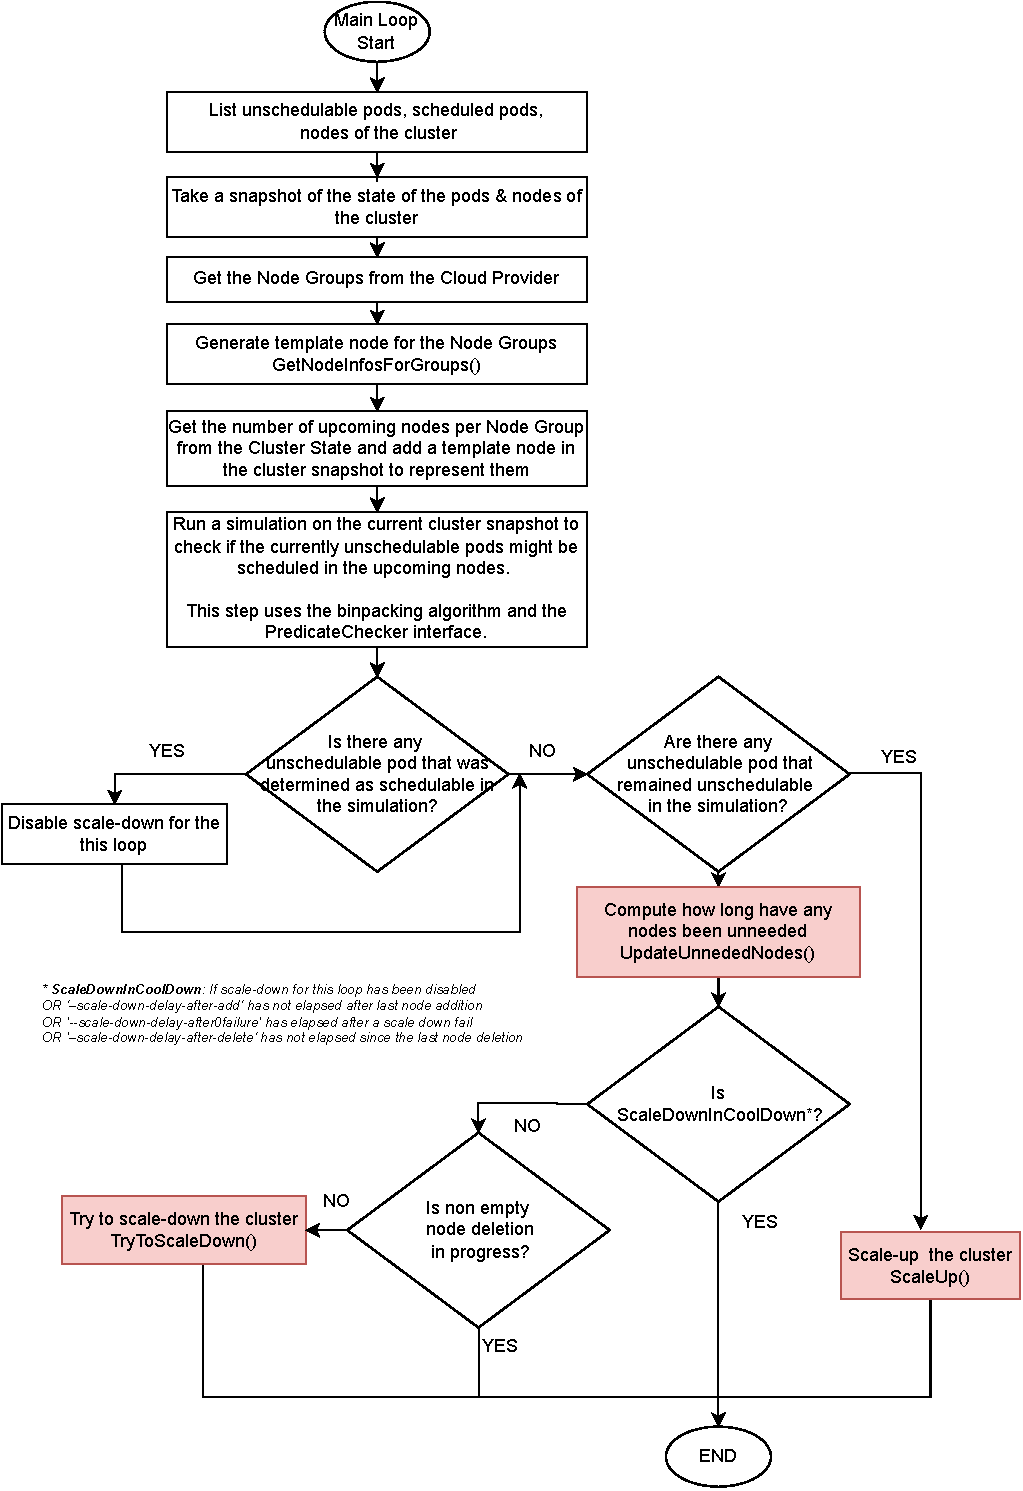
\includegraphics[width=\textwidth]{resources/autoscaler-main-loop.pdf}
      }
      \caption{Cluster Autoscaler:The main loop}
      \label{figure:autoscaler-main-loop}
\end{figure}


\subsection{Scale-Down}
\label{section:design-scale-down}
The Autoscaler tries to scale down the cluster if it did not attempt any
scale-up in the current run of the main loop. The scale-down procedure consists
of two distinct procedures:
\begin{enumerate}
      \tightlist
      \item \textit{Update unneeded nodes}: calculates which nodes have been
            unneeded and for how long.
      \item \textit{Try to scale down}: attempts to scale down the cluster by
            removing unneeded nodes.
\end{enumerate}

\begin{figure}[H]
      \centering
      \makebox[\textwidth][c]{
            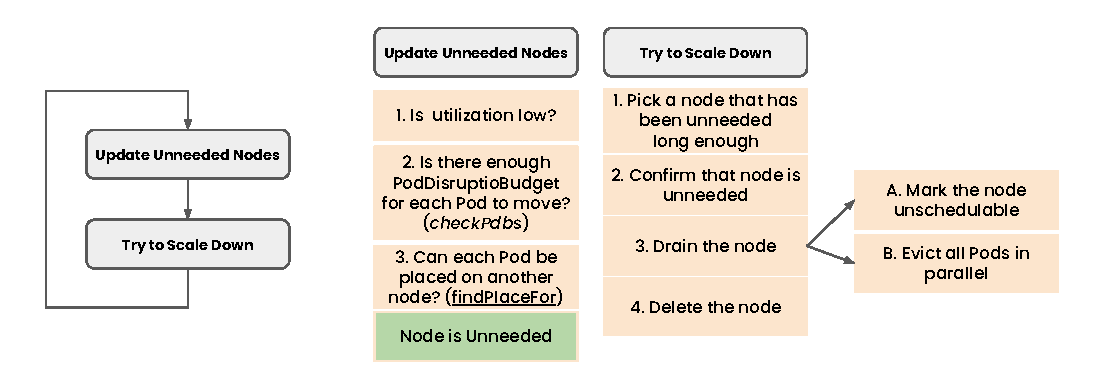
\includegraphics[width=1.1\textwidth]{resources/autoscaler-scale-down-process.pdf}
      }
      \caption{Cluster Autoscaler: Scale-down procedure}
      \label{figure:autoscaler-scale-down}
\end{figure}

We will use symbolic names to refer to various parameters of the Autoscaler in
our analysis, presented in Table \ref{table:symbolic-names-autoscaler}.
\begin{table}
      \begin{tabularx}{\linewidth}{|L|L|}
            \hline
            \textbf{Symbolic Name}        & \textbf{Description}                 \\ \hline
            scanInterval                  & How often cluster is reevaluated for
            scale up or down.
            \\
            \hline
            scaleDownDelayAfterAdd        & How long after scale up that scale
            down evaluation resumes. Defaults to 10 minutes. Configurable via
            the \co{--scale-down-delay-after-add} flag.                          \\
            \hline

            scaleDownDelayAfterDelete     & How long after node deletion that
            scale down evaluation resumes. Defaults to scanInterval.
            Configureable via the \co{--scale-down-delay-after-delete} flag.      \\
            \hline

            scaleDownDelayAfterFailure    & How long after scale down failure
            that scale down evaluation resumes. Defaults to 10 minutes.
            Configurable via the \co{--scale-down-delay-after-failure} flag.     \\
            \hline

            scaleDownUtilizationThreshold & Utilization threshold below which a
            node can be considered for scale down. Defaults to 0.5. Configurable
            via the \co{--scale-down-utilization-threshold} flag.                \\
            \hline

            scaleDownUnneededTime         & How long a ready node should be
            unneeded before it is eligible for scale down.  Defaults to 10
            minutes. Configurable via the \co{--scale-down-unneeded-time} flag.
            \\
            \hline

            scaleDownUnreadyTime          & How long an unready node should be
            unneeded before it is eligible for scale down.  Defaults to 20
            minutes. Configurable via the \co{--scale-down-unready-time} flag.
            \\
            \hline
      \end{tabularx}
      \caption{Symbolic names for various parameters of the Autoscaler used in our analysis}
      \label{table:symbolic-names-autoscaler}
\end{table}


\subsubsection{Update Unneeded Nodes Procedure}
The \textit{update unneeded nodes} procedure calculates which nodes of the
cluster have been unneeded and updates the Autoscaler's internal state with the
duration they have been unneeded. The Autoscaler considers a node
\textit{unneeded} if it meets all the following criteria:
\begin{itemize}
      \tightlist
      \item It is \textit{underutilized}, i.e., it has resource utilization
            below a specific threshold.
      \item The Pods that run on the node can be evicted (see section
            \ref{section:background-eviction}), i.e., their eviction is not
            blocked by any PodDisruptionBudgets.
      \item The Pods that run on the node can be moved to a different cluster
            node.
\end{itemize}
If a node does not meet the criteria, it is considered \textit{unremovable}.

To determine if an underutilized node is unneeded, the Autoscaler runs these
steps:
\begin{enumerate}
      \tightlist
      \item Calculate the Pods that must be moved if it removes the node.
      \item Check if any PodDisruptionBudgets block the eviction of any Pod. If
            so, the node is unremovable.
      \item Call \co{FindPlaceFor()} to find place for the Pods on a different
            node. \co{FindPlaceFor()} uses the
            \co{SchedulerBasedPredicateChecker} interface to determine if the
            Pod can be placed on any other node. It checks if the Pod can fit a
            node due to other scheduling constraints (CPU, memory), as well as
            if the Pod's volumes can be accessed from the node.
\end{enumerate}


The steps for  calculating the unneeded nodes are shown in
Algorithm~\ref{algo:update-unneeded}.

\subsubsection{Try to Scale Sown Procedure}

If a \textit{Ready} node remains unneeded for longer than
\co{scaleDownUnneededTime}, or an \textit{Unready} node remains unneeded for
longer than \co{scaleDownUnreadyTime} (see Table
\ref{table:symbolic-names-autoscaler} for the symbolic names) the Autoscaler
will consider the node as a candidate for deletion.

The Autoscaler makes a distinction between non-empty and empty nodes:
\begin{itemize}
      \tightlist
      \item \textit{Empty nodes}: nodes that run \textit{only} DaemonSet Pods.
            The Autoscaler removes them in bulk
      \item \textit{Non-empty nodes}: nodes that do not run only DaemonSet Pods.
            The Autoscaler removed them one by one to ensure that no Pods would
            be made unschedulable.
\end{itemize}

The algorithm for \co{TryToScaleDown()} is shown in
Algorithm~\ref{algorithm:try-scale-down}.

\paragraph*{Node removal} The node removal is executed as follows:
\begin{enumerate}
      \tightlist
      \item Add the \co{ToBeDeletedByClusterAutoscaler:NoSchedule} taint on the
            Node, essentially marking the node as unschedulable.
      \item Start draining the node by evicting in parallel all the Pods of the
            node. If any Pod can not be evicted due to a configured PDB, retry
            until the \co{MaxPodEvictionTimeout} exceeds.
      \item When all Pods are successfully evicted, ask the cloud provider to
            delete the node instance.
\end{enumerate}

The algorithm for the node removal is shown in
Algorithm~\ref{algorithm:node-delete}.


\clearpage
\begin{algorithm}[H]
    \caption{Cluster Autoscaler: Scale-down evaluation procedure}\label{alg:scale-down-evaluation}
    \SetKwIF{If}{ElseIf}{Else}{if~\endgraf}{\endgraf then}{else if}{else}{end if}%
    %\begin{minipage}{\textwidth}
    \begin{enumerate}[leftmargin=0cm]
        \tightlist
        \item Take a snapshot of the cluster Nodes, Pods, and PodDisruptionBudgets.
        \item \texttt{allNodes} \(\leftarrow\) List all the \co{Node} objects from the API Server.
        \item \texttt{scaleDownCandidates} \(\leftarrow\) Select nodes from
              \texttt{AllNodes} that belong to node groups that have not reached their
              minimum size.
        \item \texttt{podDestinations} \(\leftarrow\) \texttt{AllNodes};
              \texttt{podDestinations} represents the nodes that that may accept Pods in case a node is removed.
        \item Call \texttt{UpdateUnneededNodes()} with \texttt{podDestinations},
              and \texttt{scaleDownCandidates} as input, to calculate which nodes are
              unneeded an which ones are unremovable.
        \item \uIf{\begin{tabular}{@{\hspace*{1.0em}}l@{}}
                      the scale-down has been disabled for this loop                                           \\
                      % TODO: times in table
                      \textbf{OR} \co{scaleDownDelayAfterDelete} interval has not elapsed  \\
                      \textbf{OR} \co{scaleDownDelayAfterAdd} interval has not elapsed  \\
                      \textbf{OR} \co{scaleDownDelayAfterFailure} interval has not elapsed 
                  \end{tabular}}{
                  Don't scale-down the cluster. Autoscaler Status: \texttt{ScaleDownInCooldown}
              }
              \uElseIf{there is non empty node deletion in progress} {
                  Don't scale-down the cluster. Autoscaler Status: \texttt{ScaleDownInProgress}}
              \lElse{Try to scale down the cluster.}
    \end{enumerate}
    %\end{minipage}
\end{algorithm}


\begin{algorithm}[ht]
    \caption{Cluster Autoscaler: UpdateUnneededNodes() method}\label{algo:update-unneeded}
    \KwIn{\texttt{scaleDownCandidates}: a list of nodes that belong to
        node groups that have not reached their minimum size }
    \KwResult{Update the
        state of the Autoscaler with information about which nodes are unneeded}
    \begin{enumerate}[leftmargin=0.5cm]
        \tightlist
        \item For each node in \texttt{scaleDownCandidates}, call \texttt{checkNodeUtilization()}:
              \begin{enumerate}[]
                  \tightlist
                  \item \lIf{node has the ``ToBeDeletedByClusterAutoscaler'' taint}{ it is currently deleted, continue to next node}
                  \item \lIf{node has ``cluster-autoscaler.kubernetes.io/scale-down-disabled: true'' annotation}{continue to next node}
                  \item Calculate the utilization of the node.
                  \item \lIf{utilization is above threshold}{continue to next node}
                  \item Add the node \texttt{currentlyUnneededNodes}.
              \end{enumerate}
        \item \texttt{currentlyUnneededNonEmptyNodes} \lar From \texttt{currentlyUnneededNodes} select nodes that are not empty, i.e., they do not run only DaemonSet Pods.
        \item Call \texttt{findNodesToRemove(currentlyUnneededNonEmptyNodes)} to determine nodes that can be removed. For each node:
              \begin{enumerate}[]
                  \tightlist%        
                  \item Get the Pods that are running on the node and for each Pod:
                        \begin{enumerate}[leftmargin=0.5cm]
                            \tightlist
                            \item \lIf{the Pod has a Pod disruption budget that prevents its eviction}{the node is unremovable}
                            \item Call \texttt{findPlaceFor(pod)} to determine if it can be moved elsewhere.
                            \item \leIf{the Pod can not be moved elsewhere}{the
                                      node is unremovable}{the node can be removed, add it to
                                      \texttt{nodesToRemove}}
                        \end{enumerate}
              \end{enumerate}
        \item For each node in \texttt{nodesToRemove} update the state of the Autoscaler with the duration the node has been unneeded.
    \end{enumerate}
\end{algorithm}

\begin{algorithm}[ht]
\caption{Cluster Autoscaler: TryToScaleDown() method}\label{algorithm:try-scale-down}
    \KwIn{A list of unneeded nodes, as computed by UpdateUnneded() method}
    \KwResult{Scales-down the cluster}
\begin{enumerate}[leftmargin=0.5cm]
\item
  For each node in the unneeded nodes:

  \begin{enumerate}[leftmargin=0.5cm]
  \tightlist
  \item \lIf{If the node has the \texttt{cluster-autoscaler.kubernetes.io/scale-down-disabled}}{mark the node unremovable, reason \co{ScaleDownDisabledAnnotation}, go to next node.}
    \item
    \lIf{the node is \texttt{Ready}, and it has been underutilized for
    less than \texttt{ScaleDownUnneededTime}}{mark the node unremovable,
    reason \texttt{NotUnneededLongEnough}, continue to next node}
  \item
    \lIf{the node is \texttt{Unready}, and it has been underutilized for
    less than \texttt{ScaleDownUnreadyTime}}{mark the node unremovable,
    reason \texttt{NotUnreadyLongEnough}, continue to next node}
  \item
    Get the NodeGroup the node belongs to, get its \co{minSize} and current
    \co{size}, the number of node deletions in progress for the node group
    (\texttt{deletionsInProgress}).
  \item \lIf{\co{size} - \co{deletionsInProgress} $\leq$ \co{minSize}}{
    mark the node unremovable, reason \texttt{NodeGroupMinSizeReached},
    continue to next node}
  \end{enumerate}
  \item
  \co{candidates} \lar All the unneeded node that were not marked unremovable
  \item
    From \co{candidates}, try to scale-down as many as possible empty nodes.
  \item
    \texttt{nodesToRemove} \lar From the remaining candidates find nodes to
    remove (call \texttt{FindNodesToRemove()}).
  \item
    Pick a node from \texttt{nodesToRemove} and delete it
    (call \texttt{deleteNode()}) .
\end{enumerate}
\end{algorithm}
\begin{algorithm}[ht]
\caption{Cluster Autoscaler: deleteNode() method}\label{algorithm:node-delete}
    \KwIn{An unneeded Node of the Cluster to be deleted}
     \KwResult{Deletes the Node from the cluster and the Cloud Provider}
        \begin{enumerate}[leftmargin=0.5cm]
        \tightlist
        \item Add \co{ToBeDeletedByClusterAutoscaler:NoSchedule} taint on the
        Node to make the Node unschedulable.
        \item Drain the node; For each Pod (except for the DaemonSet Pods), in parallel:
            \begin{enumerate}
                \tightlist
                \item Send Eviction request
                \item \lWhile{the Eviction fails and for duration up to \co{MaxPodEvictionTimeout}}{retry the Eviction}

                Note: \co{MaxPodEvictionTimeout} is a hard-coded value equal to 2 minutes.
            \end{enumerate}
        \item \lIf{any of the Pods was not evicted successfully}{return error}
        \item \lIf{the node has any annotation with prefix
        \co{delay-deletion.cluster-autoscaler.kubernetes.io/}}{wait for up to
        \co{nodeDeletionDelayTimeout} for the annotation to be removed}
        \item Request from the Cloud Provider to delete the Node.
        \item \lIf{the Cloud Provider deletion fails}{return error}
        \end{enumerate}
\end{algorithm}


\clearpage
\subsection{Scale-Up}
\label{section:design-scale-up}
If the cluster has unschedulable Pods, the Autoscaler will try to help them by
adding new nodes to the cluster (\textit{scale-up}). A scale-up, essentially, is
the increase of the target size of one or more node groups. If multiple node
groups exist in the cluster, the cluster has to decide the following:
\begin{itemize}
      \tightlist
      \item Which node groups can help the unschedulable Pod run.
      \item How many nodes of the node group do the Pods need.
      \item If different node group scale-ups are feasible, which node group
            shall scale up.
\end{itemize}

As soon as the Autoscaler increases the target size of a node group, the cloud
provider will spin up new node instances, the new nodes will join the Kubernetes
cluster, and the scheduler will gradually scheduler the so far unschedulable
Pods to the new nodes.

The full algorithm for the \texttt{ScaleUp()} method is shown in
Algorithm~\ref{algorithm:scale-up}.

% TODO We show or is shown 
\paragraph*{Scale-up options}
To decide whether the scale-up of a node group would help the unschedulable Pod,
the Autoscaler runs the (roughly) following steps:
\begin{enumerate}
      \tightlist
      \item Take a snapshot of the cluster.
      \item Add a template node of the node group to the snapshot.
      \item Run a simulation, using the \co{SchedulerBasedPredicateChecker},
            whether the unschedulable Pod can be scheduled on the modified
            snapshot of the cluster.
      \item If the simulation determines that the Pod can be scheduled on the
            modified snapshot, use the \co{BinPackingNodeEstimator} to calculate
            how many nodes of that node group are needed.
\end{enumerate}

The option to scale up a specific node group with the number of needed nodes is
referred to as a ``\textit{scale-up option}''.

The complete algorithm to calculate a scale-up option is shown in Listing
\ref{algorithm:scaleup-options}.

\paragraph*{Scale-up strategy}

If multiple scale-up options, i.e., different node group scale-ups, can help the
unschedulable Pods, the Autoscaler decides which one is best using the
\co{Strategy} interface. There are various strategies, and the administrator can
configure the Autoscaler to use a desired one, e.g., the least cost option,
random strategy, etc.


\begin{algorithm}[ht]
    \caption{Cluster Autoscaler: ScaleUp() method}\label{alg:cap}
    \label{algorithm:scale-up} \KwIn{\co{pods}: the unschedulable Pods
        \\\co{snapshot}: the cluster snapshot } \KwResult{Adds extra nodes to
        accommodate the unschedulable Pods}
    \begin{enumerate}[leftmargin=0.5cm]
        \tightlist
        \item Build Pod equivalence groups - each Pod equivalence group consists
              of Pods that are managed by the same controller (same UUID) and have
              the same spec and labels.
        \item For each node group registered:
              \begin{enumerate}
                  \tightlist
                  \item Get its target size.
                  \item If the target size $\geq$ max size, go to the next node
                        group.
                  \item Create a template node for the node group.
                  \item Compute the expansion option for the node group, see
                        \co{ComputeExpansionsOption()}.
                  \item If any unschedulable Pod can be helped by adding a new
                        node of the node group, add the node group in the expansion
                        options list.
              \end{enumerate}
        \item If there are not any expansion options list, then do not trigger
              any scale-ups.
        \item Else, from the expansions options select one, according to the
              configured expansion strategy.
        \item Execute the selected scale up option: increase the target sizes of
              the corresponding node groups.
    \end{enumerate}
\end{algorithm}

\begin{algorithm}[ht]
    \caption{Cluster Autoscaler: ComputeExpansionsOption()
        algorithm}\label{algorithm:scaleup-options} \KwIn{\co{pods}: the unschedulable
        Pods \\\co{snapshot}: the cluster snapshot \\\co{template}: the template
        node of the node group} \KwResult{Computes if the scale-up of the node group
        would help any of the unschedulable Pods.}
    \begin{enumerate}[leftmargin=0.5cm]
        \tightlist
        \item
              For each Pod equivalence group:
              \begin{enumerate}
                  \tightlist
                  \item Get the sample Pod of the Pod equivalence group.
                  \item Add the template node in the cluster snapshot.
                  \item Call the Predicate Checker to check if any of the
                        unschedulable Pods can be scheduled in the new cluster snapshot.
                  \item If the sample Pod fits the new node in the cluster
                        simulation, append all the equivalent Pods in the list of Pods
                        that got helped (\co{options.Pods}).
              \end{enumerate}
        \item Call the bin-packing estimator to estimate how many nodes of
              the node group would be needed to help all the equivalent Pods.
        \item Return the \co{option}: a struct that indicates how many nodes of
              the node group are needed and which Pods would be helped.
    \end{enumerate}
\end{algorithm}



\clearpage
\subsection{Shortcomings \& Proposed Extensions}

In previous sections, we described the algorithms that govern the operations of
the Autoscaler; we will now identify their shortcomings.

\subsubsection{Scale-Down: Rok Volumes Can Be Migrated}
\label{section:design-autoscaler-unpinned}

When evaluating the scale-down of a node, the Autoscaler tries to find a place
for the Pods that run on the node in other cluster nodes. To do so, it calls the
\co{FindPlaceFor()} method, which in turn leverages the \co{PredicateChecker}
interface methods to determine if a Pod fits a node. The
\co{SchedulerBasedPredicateChecker} implementation of the interface runs the
VolumeBinding plugin's \co{Filter()} method to check if the volumes of the Pod
can be accessed from another node.


The PVs of the Rok storage class have node affinity that matches only with the
node where the volume was provisioned. Since the node affinity of the volumes
does not match any other in the cluster, the Autoscaler considers that the Pod
and its volume can not be moved on a different node, thus, marking the current
node as unremovable. The \co{SchedulerBasedPredicateChecker} does not know that
the Rok volumes have a mechanism to snapshot and recover them on a different
node [by unpinning them (snapshot + remove volume's node affinity, see section
            \ref{section:design-unpin}) and then pinning them (restoring the data) on
            another node ].

We propose the extension of the Autoscaler to simulate the Rok volumes as
unpinned (as if they do not have node affinity) when evaluating a scale-down
(and only then; in other cases, the volumes are retaining their node affinity).
With this extension, the Autoscaler will comprehend that the Rok volumes can
move anywhere in the cluster, and it can remove the node safely.

\subsubsection{Scale-Down: Coordinate With the Rok CSI Guard Mechanism}

As part of the Rok volume protection mechanism (see section
\ref{section:background-rok-csi-guard}), we deploy a \texttt{Deployment} object
for each node of the cluster, which creates a Pod per node (Rok CSI Guard)  with
strict node affinity that matches only the node it protects. The Autoscaler
tries \textit{to find place} to move this Pod. Since the Pod has strict node
affinity that matches only the current node, SchedulerBasedPredicateChecker
assumes that the Pod cannot be moved to a different node. Because of that, the
Autoscaler marks the node as unremovable. Of course, the Rok Operator will
remove the Pod after the Autoscaler removes the node, but the Autoscaler is
unaware of this fact.

Moreover,  the Autoscaler checks the PDB of the Guard Pod. The PDB of the Guard
Pod is configured to cause any evictions to fail. The Autoscaler notices that
and assumes that the Guard Pod will not be able to get safely evicted, thus,
marking the node unremovable. It is unaware that the Rok Operator will remove
them as soon as the scale-down starts and the Rok CSI  unpins all the local
volumes of the node.

We propose the extension of the Autoscaler so that it does not try to find a
place for the operator-managed ephemeral Guard Pods. Moreover, we extend the
Autoscaler to ignore the PDB of the Guard Pod. Still, the Autoscaler will be
aware that the Guard Pod exists, evicting it when it drains the node. This
eviction will fail as long as the PDB exists and the Autoscaler will retry,
delaying the deletion of the node.

To make things more obvious, here is the procedure that will take place with the
new design:


\begin{enumerate}
      \tightlist
      \item The Autoscaler evaluates a node for removal:
            \begin{enumerate}
                  \item It checks if the PDB allows the eviction of the Pods
                        running on the node, but it ignores the PDB of the Guard
                        Pod.
                  \item It tries to find a place for each Pod on a different
                        node, but it ignores the Guard Pod.
            \end{enumerate}
      \item The Autoscaler decides to remove the node.
      \item The Autoscaler adds the deletion taint on the node, effectively
            marking it as unschedulable for Pods.
      \item The Autoscaler sends eviction requests for each Pod to the API
            Server.
      \item The eviction of all the Pods --except for the Guard Pod-- succeeds.
      \item The Autoscaler keeps retrying to evict the Guard Pod, but the API
            Server responds that the eviction is not allowed due to the
            configured PDB.
      \item The Rok CSI Controller notices that the node is unschedulable and
            that no workload mounts the volumes, so it starts unpinning them.
      \item The Rok CSI Controller finishes the unpinning of the PVs.
      \item The Rok Operator removes the PodDisruptionBudget of the Guard Pod.
      \item The Autoscaler's request to evict the Guard Pod succeeds since the
            PDB was removed.
      \item The Autoscaler asks the cloud provider to delete the node.
      \item The Rok Operator removes the Rok CSI Guard \texttt{Deployment}
            object that corresponds to the removed node.
\end{enumerate}

Let us notice that the Autoscaler keeps retrying the eviction of the Guard Pod
for up to 2 minutes. That duration is a hard-coded timeout that might not be
enough in most cases. Taking a snapshot of the volume may last more than 2
minutes, depending on the size of the volume. It would be wise to use more sane
values and allow the user to cluster's admin to configure the value when
deploying the Autoscaler. To do so, we propose the extension of the Autoscaler
with a flag to configure the max pod eviction timeout.

\label{section:design-autoscaler-guards}


\subsubsection{Scale-Down: Consider Storage Capacity}

The Autoscaler shall check if the Rok volumes of a Pod can fit a node concerning
their requested storage capacity when evaluating a scale-down. As we have
explained, the Autoscaler used the \texttt{SchedulerBasedPredicateChecker}
interface in order to check if a Pod fits a node, which --among others-- calls
the VolumeBinding plugin's \co{Filter()} method.

We propose the extension of the SchedulerBasedPredicateChecker's VolumeBinding
plugin's \co{Filter} method: When evaluating if a Pod can be moved to a
different node, check if there is enough available storage on the node to move
the volumes.

Moreover, since the snapshotting and migration of a volume is a procedure that
costs in terms of time, the  Autoscaler shall not remove nodes with high storage
utilization, similarly to how it handles the CPU and memory resources. To
achieve this, we propose the extension of the Autoscaler with a new metric,
called the (Rok) ``\textit{storage utilization}'', defined as the ratio of the
used storage over the max storage capacity of the node. The Autoscaler will
compare this metric against a threshold configurable by the admin via a
corresponding flag; if the storage utilization exceeds the threshold, the node
will be considered unremovable.

\subsubsection{Scale-Down: Do Not Remove Unready Nodes}

A node that with status \co{Ready} can become \co{Unready} (or \co{NotReady}) if
a system problem on the node arises. Common reasons include lack of resources on
the node, a problem with the kubelet, an error related to kube-proxy, or a
networking problem in general.

The Autoscaler removes any unneeded Unready node after the
\texttt{scaleDownUnreadyTime} elapses. In the case of local volumes, we assume
that the node will always be in good condition, with all the systems up and
running and having network access, so Rok snapshots the local volumes to
Amazon's S3 remote storage. If that does not hold, removing a node will probably
cause any local data to be permanently lost.

The Autoscaler must not remove Unready nodes. The Unready nodes shall remain in
the cluster so that an administrator takes action to recover them from the
Unready state. We propose the extension of the Autoscaler with a flag to
explicitly disable the scale-down for nodes in \co{Unready} state and consider
them unremovable.

\subsubsection{Scale-Up: Consider Storage Capacity}
The Autoscaler does not know how much local storage is available when a new node
is spanned up and added to the cluster. The template node it creates from a live
node contains information only for the \textit{currently} free storage (of the
live node), reported on the capacity annotation by the storage driver (see the
proposed scheduler design, section \ref{section:capacity-annotation}). We need a
mechanism to know how much free storage a new node of a node group will have,
and the Autoscaler shall consider it in its simulations.

\paragraph*{Report max capacity}
Assuming that all the nodes in a node group have the same disk configuration and
max storage capacity, we can use the storage driver to report what the new
node's storage capacity would be on the \co{Node} objects. We propose the
extension of the Rok CSI Node component to report the max capacity of a node as
a label on the \co{Node} object. This label will be referred to as the
``\textit{max capacity label}'' \footnote{The \textit{Rok max capacity label}:
      rok.arrikto.com/max-instance-capacity}.

We use a label instead of an annotation because various cloud providers give the
cluster admins the option to pass labels to the node group node templates the
cloud provider plugin constructs. In case no live node for the node group
exists, the Autoscaler will construct the template from the cloud provider
plugin and have the configured admin labels on it.

At this point, let us distinguish the two reported quantities:
\begin{itemize}
      \tightlist
      \item \textit{capacity annotation}: the remaining free storage of a live
            node. The storage driver reports it, and the scheduler considers it
            when scheduling Pods.
      \item \textit{max capacity label}: the max storage capacity of the live
            node. i.e., the total storage capacity. That is a time constant
            value that depends on the node's disks.
\end{itemize}

For example, a node might have 200 Gi total storage (reported on the max
capacity label), and only 100 Gi out of them are free (reported on the capacity
annotation).

\paragraph*{Pass the max capacity information to the template}

For the Autoscaler to simulate the scheduling with capacity considerations, we
will import in the SchedulerBasedPredicateChecker the extended VolumeBinding
(see section \ref*{section:volume-plugin-extensions}).

The extended VolumeBinding plugin will look for the capacity of a template node
on the capacity annotation and not on the label. Since the template will get the
annotation from a live node, it will represent the currently free storage on the
live node instead of the max storage capacity. We need to sanitize the value and
set it to the actual max capacity. To do so, we propose the extension of the
sanitization mechanism of the Autoscaler to copy the max capacity label's value
to the capacity annotation. In this way, the template node's capacity annotation
will indicate the max capacity (total) storage of the new node of the node
group.

The sanitization mechanism shall set the capacity annotation to an infinitely
large value if the max capacity label does not exist. This design choice offers
the following advantages:
\begin{enumerate}
      \item The Autoscaler treats the node as if it had infinite storage
            capacity and will add a live node of the node group (scale-up). If
            the decision was wrong (\textit{false scale-up}), i.e., the added
            node does not have enough storage capacity for the Pod that
            triggered the scale-up, the scheduler of the cluster will not assign
            the Pod to the newly added node. As a result, the node will remain
            unneeded, and the Autoscaler will remove it after some time. The
            system will gradually fix the wrong decision.
      \item The wrong node addition allows the Autoscaler to learn the actual
            max capacity of the node. The Rok CSI driver gets the chance to run
            on the node, and the Autoscaler generates a template node from the
            live node, which contains accurate information for the max available
            capacity reported by the Rok CSI driver.
\end{enumerate}


\paragraph*{Wait for Rok CSI to run}

If a Pod triggers a scale-up because of the storage it requests, it may take a
reasonable time from the node addition till the Rok CSI driver starts running on
the node. As long as the Rok CSI is not running on the node, the corresponding
capacity annotation is not set on the \co{Node} object. The scheduler does not
schedule the Pod on the node since the absence of the annotation indicates the
storage is unavailable (see Section ~\ref{section:design-volume-binding}). The
Autoscaler runsthe scheduling simulation and decides that the Pod does not fit
the newly added node (since the live node has no capacity annotation), so it
triggers a new scale-up.

To resolve this issue, the Autoscaler must wait for the Rok CSI driver to run on
the newly added node. As long as the driver does not run on a new node (i.e.,
the node does not have the capacity label set), the Autoscaler shall replace the
node with an \textit{Unready} copy.

The Autoscaler treats Unready nodes as upcoming nodes (for a duration of up to
15 minutes): it replaces them with template nodes of the node group they belong
to in its simulations. The template node will have the capacity annotation set
as if the Rok CSI was running. The Autoscaler's simulation will assume that Pod
will be scheduled on the node when the Rok CSI is ready and running and will not
trigger any further scale-up.

We mentioned that the Autoscaler treats Unready node as upcoming for up to 15
minutes. That needs a bit of explanation. The Autoscaler gives the nodes a
reasonable amount to become fully Ready; after this duration, it will stop
replacing the Unready nodes with their template and will consider them
unschedulable in the simulation. If any Pods that relied on the node becoming
ready (in order to run there) still exist, they will now trigger another
scale-up. Of course, in the case of Rok, 15 minutes are more than enough for the
Rok CSI driver to become ready and start running.

